\documentclass[12pt]{report}
\usepackage[utf8]{inputenc}
\usepackage[myheadings]{fullpage}

% Package for headers 
\usepackage{fancyhdr}
\usepackage{lastpage}
\usepackage{titlesec}
  
% For figures and stuff
\usepackage{graphicx, wrapfig, subcaption, setspace, booktabs}
\usepackage[T1]{fontenc}

% Change for different font sizes and families
\usepackage[font=small, labelfont=bf]{caption}
\usepackage{fourier}
\usepackage[protrusion=true, expansion=true]{microtype}

%% line and paragraph spacing
% \linespread{1.0}
\setlength{\parskip}{1em}
% \titlespacing{\section}{0pt}{2.5ex plus 1ex minus .2ex}{1.3ex plus .2ex}

% Maths
\usepackage{amsmath,amssymb}
\usepackage{float}
\usepackage{graphicx}
\usepackage{wrapfig}
\usepackage[colorinlistoftodos]{todonotes}
\usepackage[colorlinks=true, allcolors=blue]{hyperref}

% % Bibliography
\usepackage{biblatex} 
\addbibresource{references.bib}

%% Language and font encodings
\usepackage[english]{babel}

% % code
% Better inline directory listings
\usepackage{listings}
\usepackage{xcolor}
\definecolor{light-gray}{gray}{0.95}
\newcommand{\code}[1]{\colorbox{light-gray}{\texttt{#1}}}
\definecolor{codegreen}{rgb}{0,0.6,0}
\definecolor{codegray}{rgb}{0.5,0.5,0.5}
\definecolor{codepurple}{rgb}{0.58,0,0.82}
\definecolor{backcolour}{rgb}{0.95,0.95,0.92}

\lstdefinestyle{mystyle}{
    backgroundcolor=\color{backcolour},   
    commentstyle=\color{codegreen},
    keywordstyle=\color{magenta},
    numberstyle=\tiny\color{codegray},
    stringstyle=\color{codepurple},
    basicstyle=\ttfamily\footnotesize,
    breakatwhitespace=false,         
    breaklines=true,                 
    captionpos=b,                    
    keepspaces=true,                 
    % numbers=left,                    
    % numbersep=5pt,                  
    showspaces=false,                
    showstringspaces=false,
    showtabs=false,                  
    tabsize=4
}

\lstset{style=mystyle}

\newcommand{\HRule}[1]{\rule{\linewidth}{#1}}
\onehalfspacing
\setcounter{tocdepth}{5}
\setcounter{secnumdepth}{5}

%% Sets page size and margins
\usepackage[a4paper,top=2cm,bottom=1.5cm,left=2cm,right=2cm,marginparwidth=1.5cm]{geometry}

% Enable header and footer 
\pagestyle{fancy}
\fancyhf{}

% Header and footer information
\setlength\headheight{15pt}
\fancyhead[L]{ECE 5725 \- Lab2} 
\fancyhead[R]{Yu Zhang\quad}
\fancyfoot[R]{\thepage}

\setlength{\parindent}{0pt} 

\begin{document}

\date{}

% Do not change anything here except in \LARGE \textbf{This is the title of the essay} 
% /hline before and after the title makes those horoziontal lines appear, you can change the appearance by changing the 2pt to different sizees
\title{ \normalsize {\textbf{Cornell University}}
		\\ [1.0cm]
		% Change to your faculty if needed
		
\includegraphics[width=25mm]{img/cornell_logo.png}\\[.5cm]
		Electrical & Computer Engineering \\
		\HRule{2pt} \\
		\LARGE \textbf{ ECE 5725 - Embedded Operating System} \\%para que quede encerrado en las lineas
		\LARGE {\color{blue}{\textbf{LAB2 Report}}}
		\HRule{2pt} \\ [0.5cm]
		\normalsize \ {Lab Section: \textbf{Monday} }\\
% 		\normalsize \today \vspace*{5\baselineskip}
		\normalsize \ {Lab Date: 09/23/21 \And 09/27/21} \vspace*{5\baselineskip}\\
		}
		
\author{
		{ \textbf{Yu Zhang \quad yz2729}}\\[5cm]
		\large {\textbf{\today} } 
		}
		

\maketitle
%\newpage

% Uncomment the next line if you want keywords/index terms after the abstract. 
%\textit{\textbf{Keywords}: lorem, ipsum, dolor}
\section*{1. Introduction\vspace{-1em}}
In this lab, I first learned how to add external buttons to the Raspberry PI and apply callback functions to control playing the video. After that, I learned how to configure and use the piTFT screen on which I developed programs with the Pygame library.\vspace{-1em} 
\section*{2. Design and Testing\vspace{-1em}}
In this section, I will introduce my experimental process step by step and describe in detail the phenomena and problems I encountered, the solutions and the final results.\vspace{-1em}
\subsection*{2.1 Add External Buttons}
The start of this lab is to add more buttons to the Raspberry Pi. I first need to use the Breadboard, some resistors and wires to complete a circuit. The final result is shown in figure \ref{fig:fig1}.\par
From figure \ref{fig:fig1}, it can be easily find that I have used the GPIO 26 pin and GPIO 19 pin as our input source and used the pull up resistor to protect GPIO pins. 
\begin{figure}[H]
    \centering
    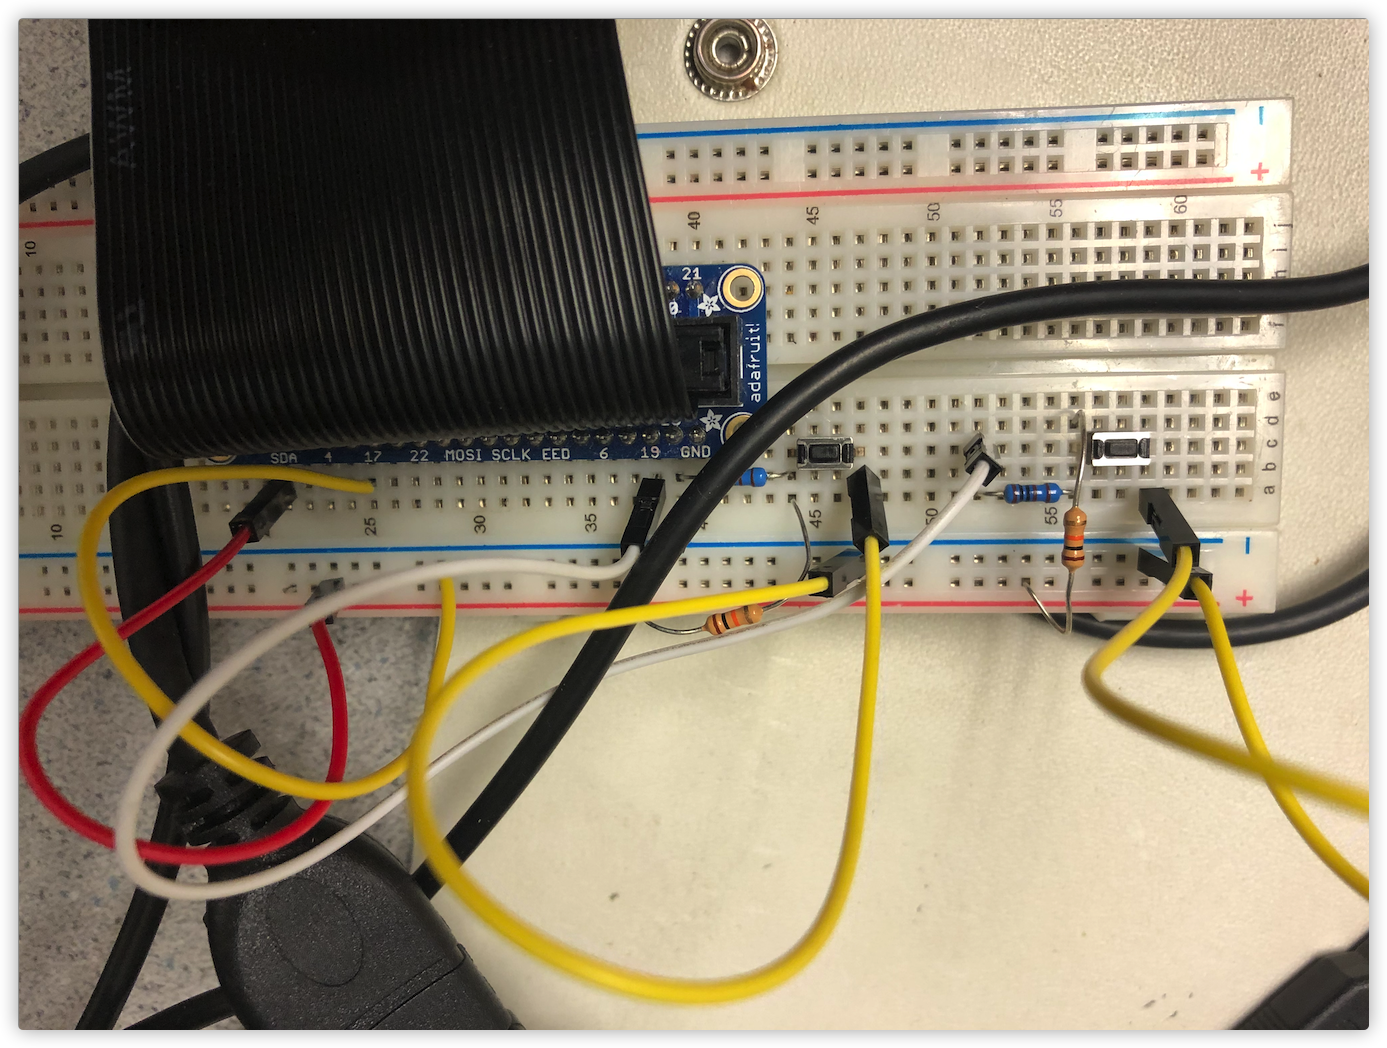
\includegraphics[width=\textwidth]{img/Circuit.png}
    \caption{The final Circuit}
    \label{fig:fig1}
\end{figure}
In order to test if my circuit is connected correctly and works properly, after asking the professor to check the circuit for me, I started writing the program \code{six\_button.py} to check the function of all the buttons. The complete code is shown in the Apendix. Here, I only focus on the settings for GPIO 26 and GPIO 19. In two lines of code shown in the code listing \ref{code:code1}, I set up the GPIO 26 pin and the GPIO 19 pin as GPIO.IN mode and the third parameter was set to be \code{GIPO.PUD\_UP} as I used a 10k resistor as the pull-up resistor and 1k resistor to protect GPIO pins.
\begin{center}
\begin{lstlisting}[language=Python, caption= Setup codes for two more button, label=code:code1] 
# Add two more button 
GPIO.setup(26, GPIO.IN, pull_up_down=GPIO.PUD_UP)
GPIO.setup(19, GPIO.IN, pull_up_down=GPIO.PUD_UP)
\end{lstlisting}
\end{center}\vspace{-2em}
After running the program \code{six\_buttons.py} to confirm that all six keys were detected properly, I started to expand the original program \code{video\_control.py} to create \code{more\_video\_control.py} and added two more keys to the it. A button would fast forward the video for 30 seconds and another would rewind the video for 30 seconds. The logic for writing these functions is the same as the previous ones, they all pass a corresponding command to the FIFO file after detecting the corresponding key press event.\par
HoIver, during the actual testing of the program \code{more\_video\_control.py}, I found that sometimes I only pressed a key once, but the corresponding function ran twice or even three times. Other times, I pressed the button but it did not respond. To solve this probelm, I set the bounce time to 500. After the modification, the stability of the program has been substantially improved.\par
Then, I successfully modified the original shell script \code{start\_video} to run the program \code{more\_vid} \code{eo\_control.py} with the \code{mplyar} application. The complete code of \code{start\_video} and  \code{more\_vid} \code{eo\_control.py} are shown in the Apendix.\par
At this point I finished the first part of this lab, with a complete and workable circuit and the basic Python program. Next, I would change the polling loop method to the callback function for triggering the interruption.\vspace{-1em}
\subsection*{2.2 Interrupt Callbacks and Performance Measurement}\vspace{-1em}
In this section, I need to modify the  \code{more\_video\_control.py} to the  \code{more\_video\_control\_cb.py}, which apllied the callback functions to detect button press event and trigger the interruption. Then, I need to measure the performance for both two Python programs and record performance result of \code{more\_video\_control.py} with different polling frequency.\par
In fact, the method to introduce the callback functions is very easy. The initialization settings of GPIO pins are still the same as mentioned in the last section, set to GPIO.IN mode, and set to pull-up resistor. The difference is that for every GPIO pin I would assign a callback function by using the function \code{GPIO.add\_event\_detect()}. Our complete code of \code{more\_video\_control\_cb.py} is shown in the Apendix. Here, I take GPIO 26 as an example and give its sample code in code listing \ref{code:code2}.\par 
\begin{center}
\begin{lstlisting}[language=Python, caption=Sample code for GPIO 26, label=code:code2]
# the callback function for GPIO 26
def GPIO_26_callback(channel):
    print("Button 26 has been pressed") 
    cmd = 'echo "seek 30 " > /home/pi/video_fifo'
    print("Fast forward 30 seconds")
    os.system(cmd)
if __name__ == '__main__':
    # setup the GPIO 26
    GPIO.setup(26, GPIO.IN, pull_up_down=GPIO.PUD_UP)
    # add event for GPIO 26
    GPIO.add_event_detect(26,GPIO.FALLING, callback=GPIO_26_callback,\ 
                      bouncetime=500)
    time.sleep(120)
    GPIO.cleanup()
\end{lstlisting}
\end{center}\vspace{-2em}
In the callback function \code{GPIO\_26\_callback(channel)}, I defined that if the button connected to the GPIO 26 pin was pressed, the program would pass the fasting forward command to the FIFO file. In the \code{GPIO.add\_event\_detect()} function, I specified four parameters, like GPIO pin number, the event, the callback function and the bounce time. The event \code{GPIO.FALLING} means the change in state of an electrical signal from HIGH to LOW (falling edge). In this case, it means that the button has been pressed. The bounce time means that the time between our detection. In our code, I set the bounce time to 500, which means that any key presses generated 500 milliseconds after a key press is detected will be ignored.\par
Instead of using a polling loop, I directly let the program sleep for 120 seconds. During this program sleeping, if a button press was detected, the sleep would be interrupted and then the program would execute the corresponding callback function. Using our sample code as an example, once the button connected to the GPIO 26 pin is pressed, the program will jump to the callback function \code{GPIO\_26\_callback(channel)} and execute its content. So, the video will be fasted forward 30 seconds if I press the button.\par
Following the logic I described above, I successfully completed the program \code{more\_video\_contr}\\\code{ol\_cb.py}. Next, I first need to configure the \code{perf} tool and then use it to test the performance of these programs.\par
To correctly install the package for the \code{perf} tool, I should execute the command \code{sudo apt-get }\\\code{install linux-perf-4.18}. If I don't make any changes, I must have to execute the command like \code{perf\_4.18 parameters} every time. Because if I execute \code{perf} directly, the system will return us an error, "linux-perf-5.10 is not installed". To fix this problem, I need to take a glance at the file \code{/usr/bin/perf} and make some modification. The original version is shown in the code listing \ref{code:code3}. If I execute the command \code{uname -r}, I can get the result "5.10.17-v7l+". That's why our system thinks the \code{perf} version is 5.10. The solution to this problem is also very simple, I directly comment out the code to get the version and assign the version to 4.18. After this modification, I can run the \code{perf} command normally without errors. In our experiments, I created a simple Python program \code{cal\_v1.py} to test if \code{perf} worked correctly. The test result is that it worked fine.
\begin{center}
\begin{lstlisting}[language=bash, caption=The original version, label=code:code3]
#!/bin/bash
# Execute the right version of perf for the current kernel.
# Remove flavour or custom suffix and fix number of version components to 2.
version="$(uname -r)"
version="${version%%-*}"
case "$version" in
    *.*.*)
       version="${version%.*}"
       ;;
esac
shopt -s execfail
exec "perf_$version" "$@"

# Not found? Tell the user which package to install.
case "$version" in
    3.* | 4.0 | 4.0.*)
        package=linux-tools-$version
        ;;
    *)
        package=linux-perf-$version
        ;;
esac
echo >&2 "E: $package is not installed."
exit 1
\end{lstlisting}
\end{center}\vspace{-2em}
After installing, configuring and testing \code{perf}, and making sure everything was correct, I started measuring the performance of our two python programs,  \code{more\_video\_control.py} and \code{more\_vi}\\\code{deo\_control\_cb.py}. The results of them are separately shown in the figure \ref{fig:fig2} and figure \ref{fig:fig3}. The command I used was \code{sudo perf\_4.18 stat -e task-clock, context-switches, cpu-mi}\\\code{grations, page-faults python SCRIPTNAME.py}. 
\begin{figure}[H]
\centering
\begin{minipage}[t]{0.48\textwidth}
\centering
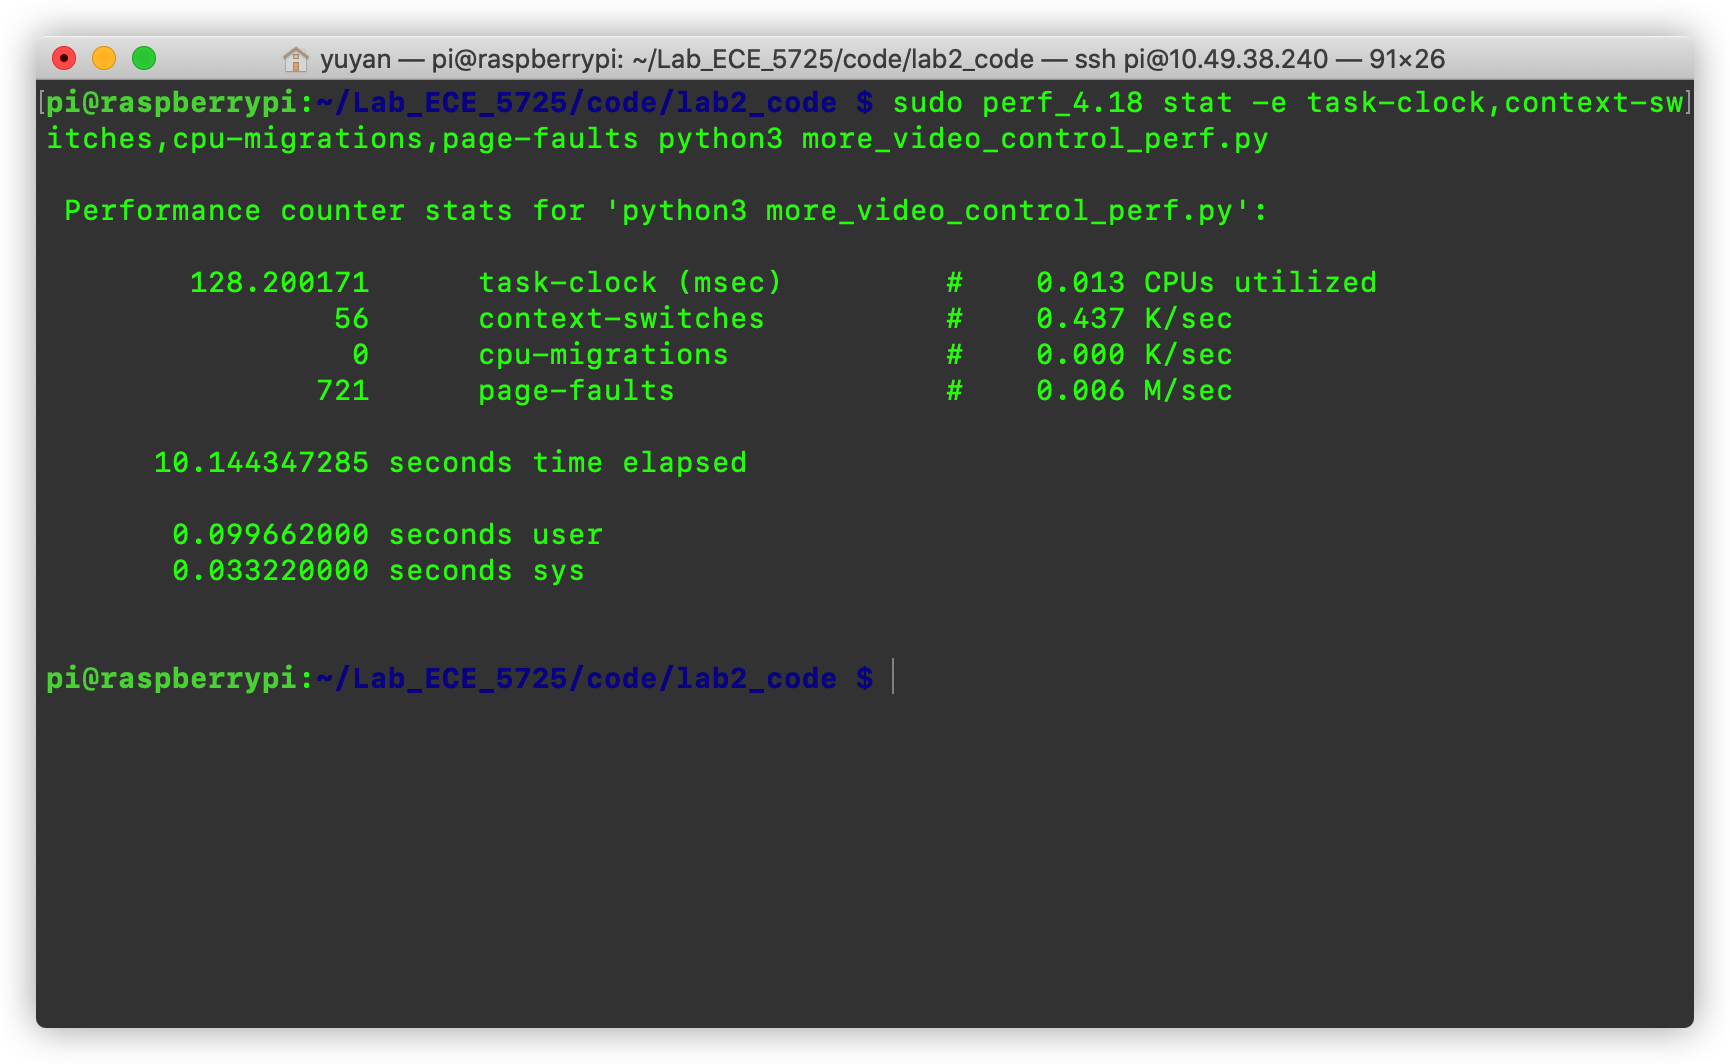
\includegraphics[width=\textwidth]{img/more_video_control_perf.png}
\caption{Performance of more\_video\_control.py}
\label{fig:fig2}
\end{minipage}
\begin{minipage}[t]{0.48\textwidth}
\centering
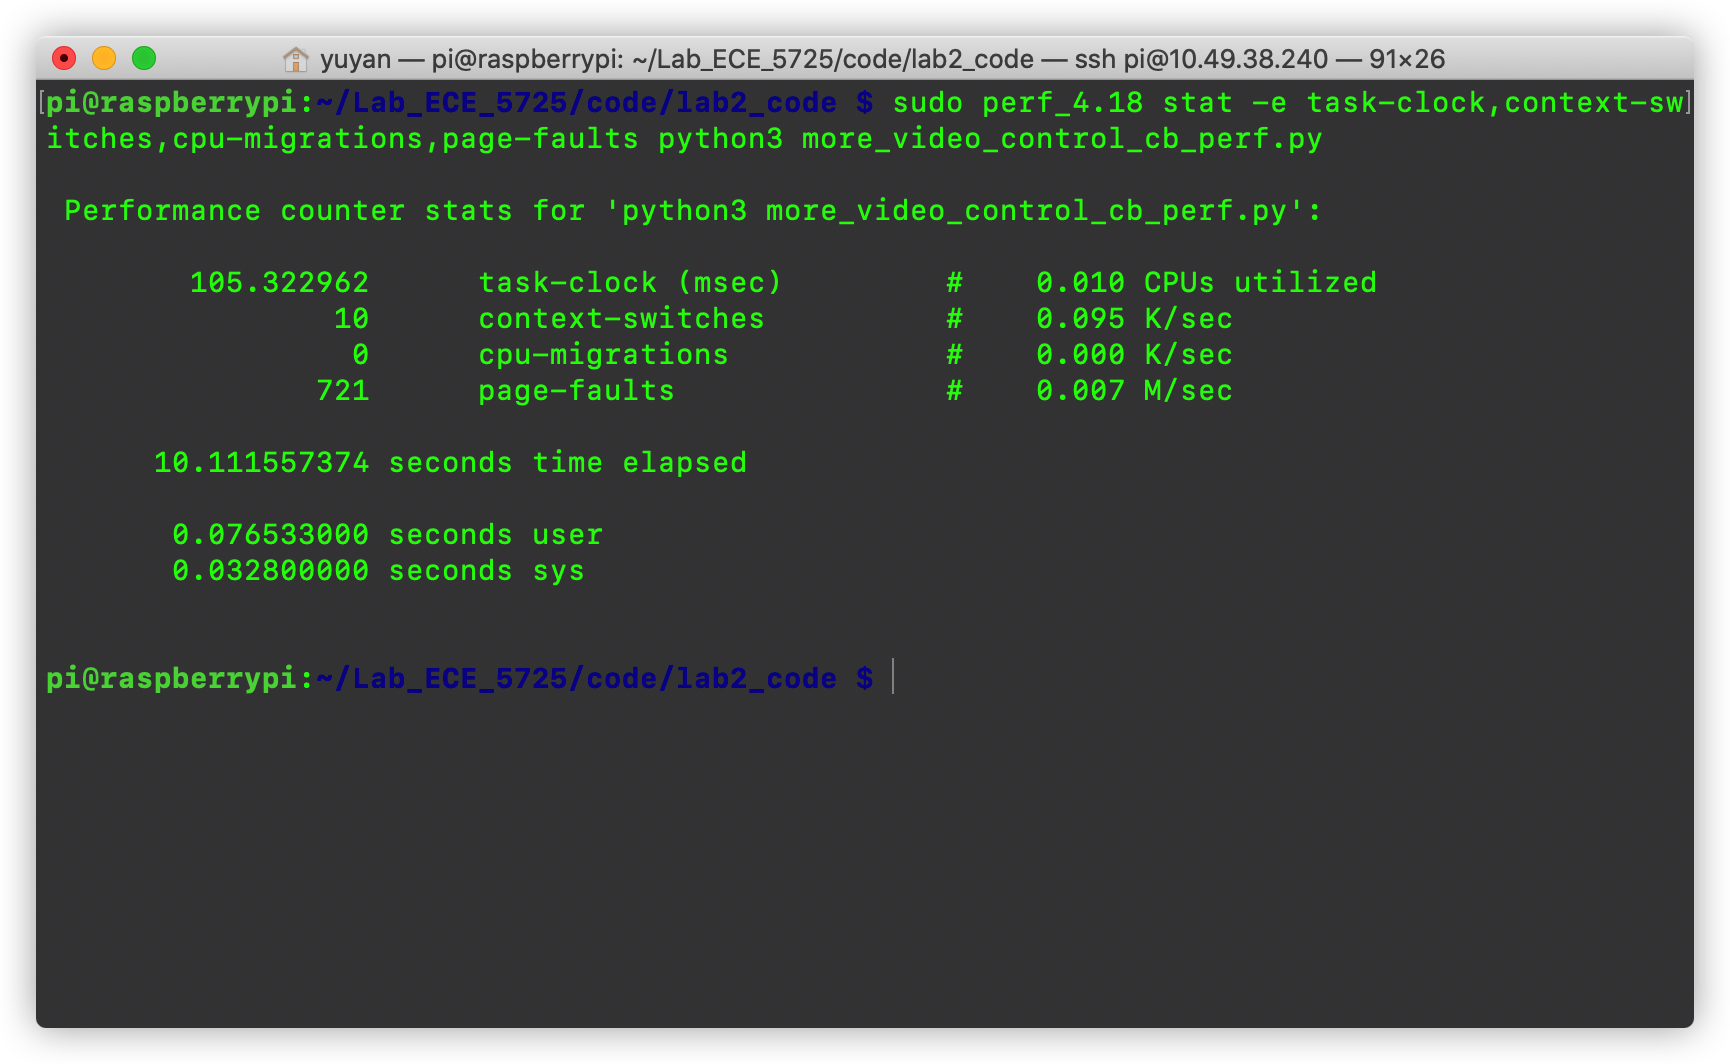
\includegraphics[width=\textwidth]{img/more_video_control_cb_perf.png}
\caption{Performance of more\_video\_control\_cb.py}
\label{fig:fig3}
\end{minipage}
\end{figure}
In these two figures, I can't really see much of a performance gap. Because I set \code{time.sleep()} to 0.2 seconds in program \code{more\_video\_control.py}, it doesn't poll as much, so it doesn't take up a lot of CPU resources in comparison. Next, I would modify the polling time into 20 milliseconds, 2 milliseconds, 200 microseconds, 20 microseconds and 0. There results are shown from figure 4 to figure 8.
\begin{figure}[H]
\centering
\begin{minipage}[t]{0.48\textwidth}
\centering
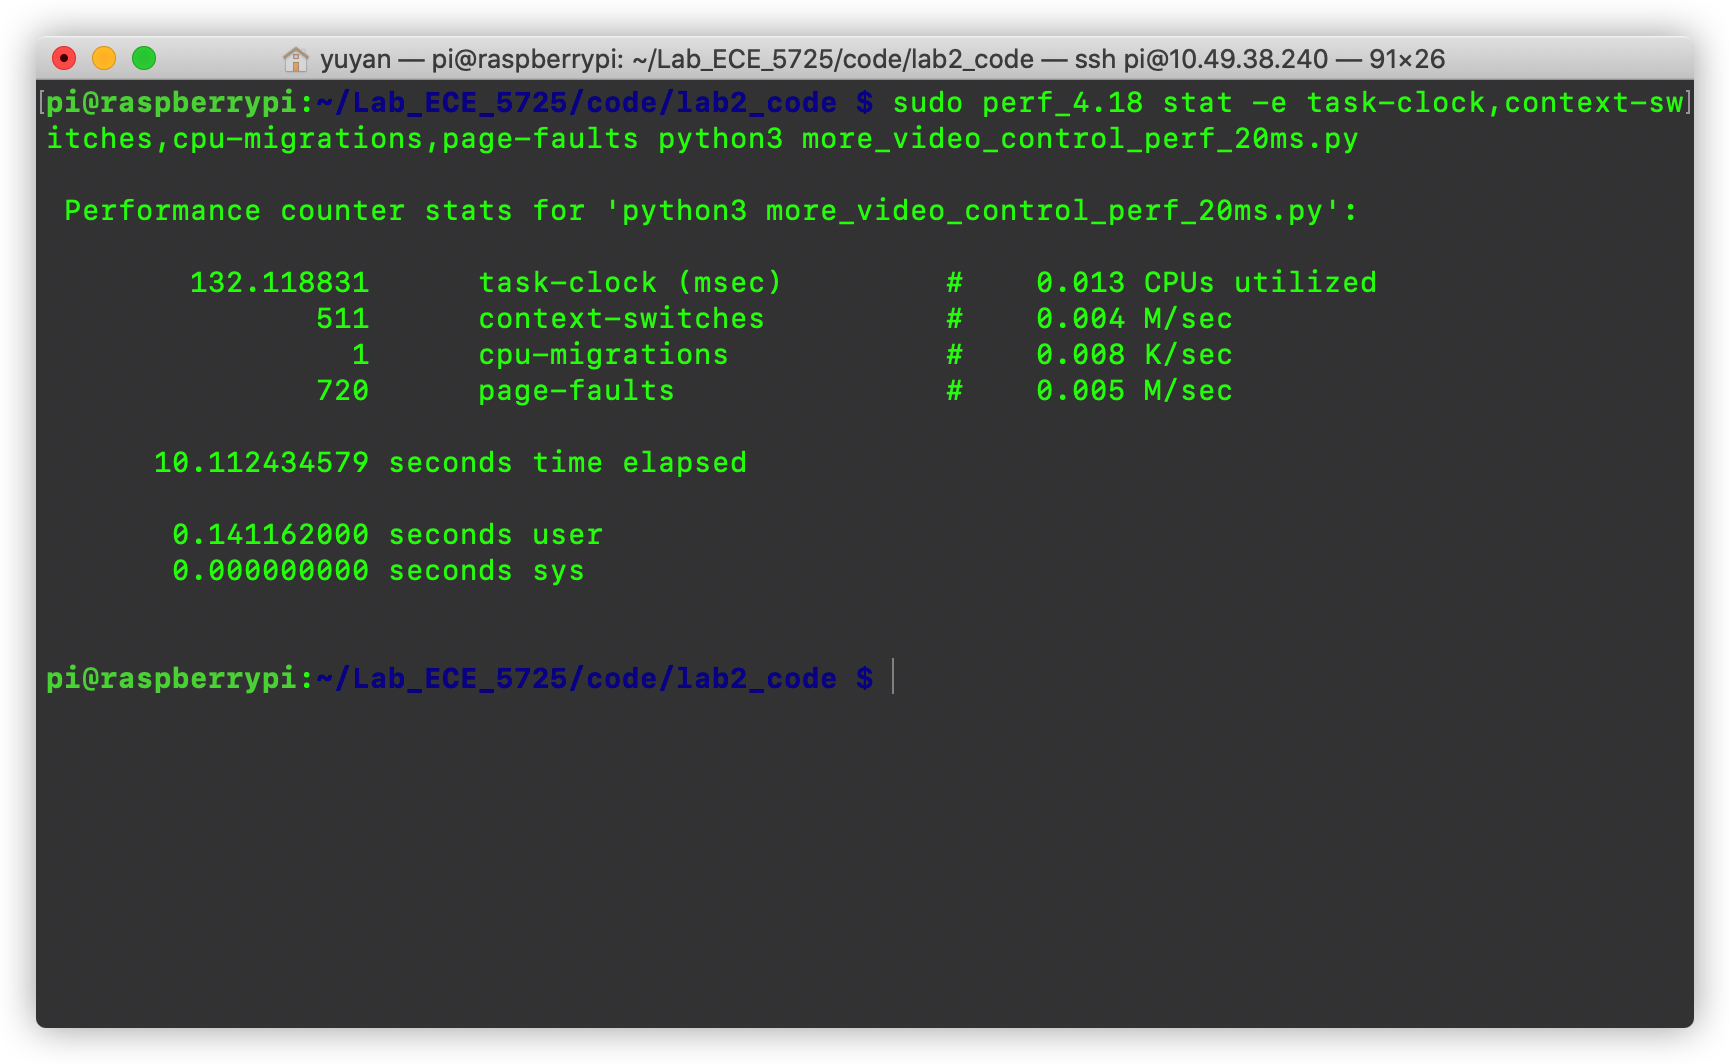
\includegraphics[width=\textwidth]{img/more_video_control_perf_20ms.png}
\caption{Performance of 20 milliseconds}
\label{fig:fig4}
\end{minipage}
\begin{minipage}[t]{0.48\textwidth}
\centering
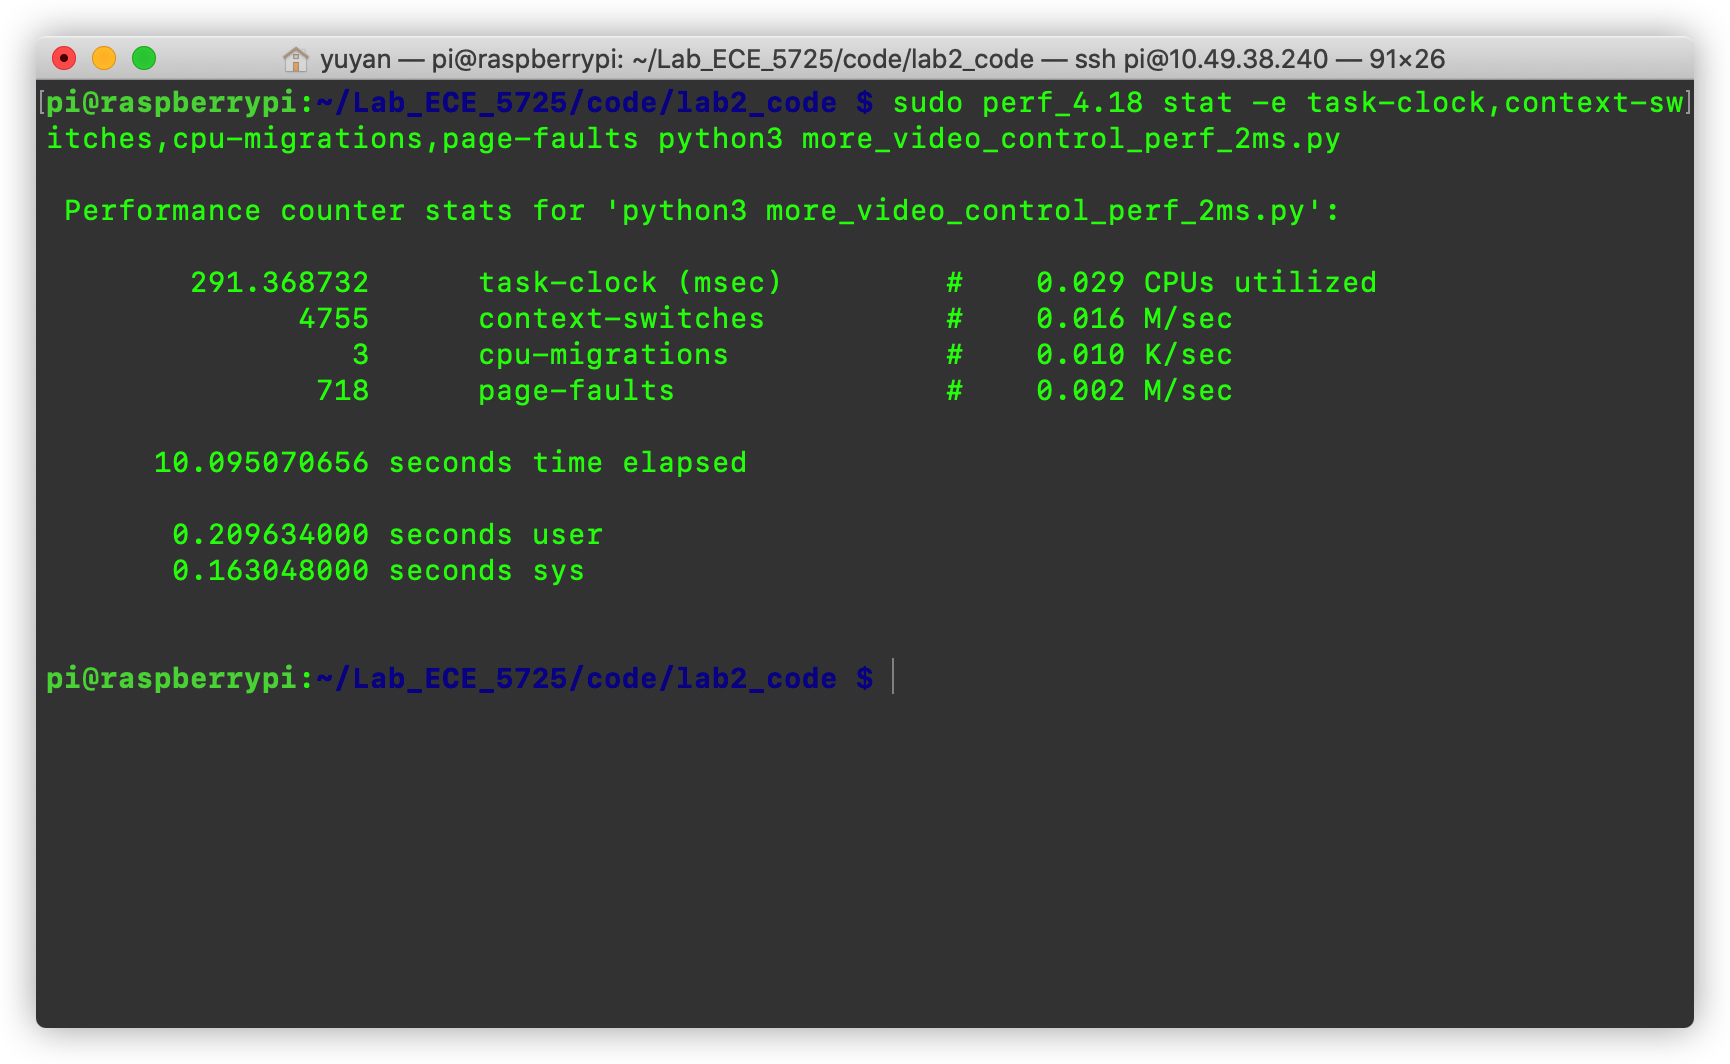
\includegraphics[width=\textwidth]{img/more_video_control_perf_2ms.png}
\caption{Performance of 2 milliseconds}
\label{fig:fig5}
\end{minipage}
\end{figure}
\begin{figure}[H]
\centering
\begin{minipage}[t]{0.48\textwidth}
\centering
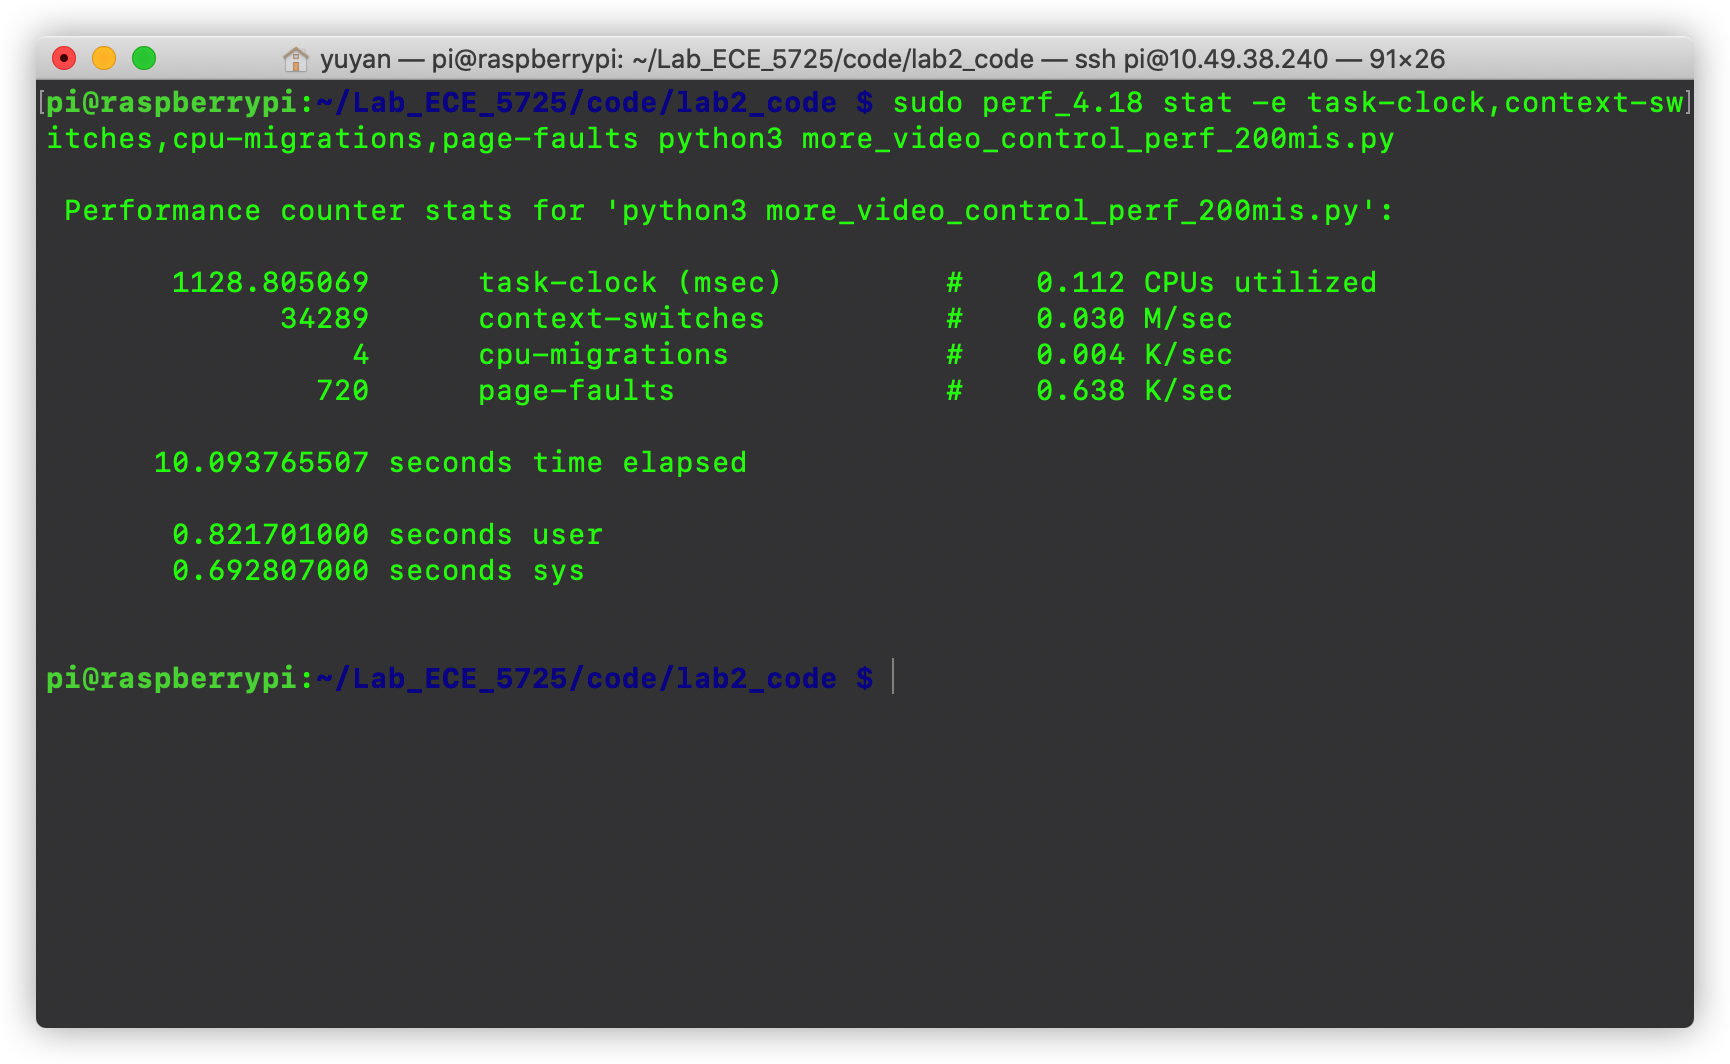
\includegraphics[width=\textwidth]{img/more_video_control_perf_200mis.py.png}
\caption{Performance of 200 microseconds}
\label{fig:fig6}
\end{minipage}
\begin{minipage}[t]{0.48\textwidth}
\centering
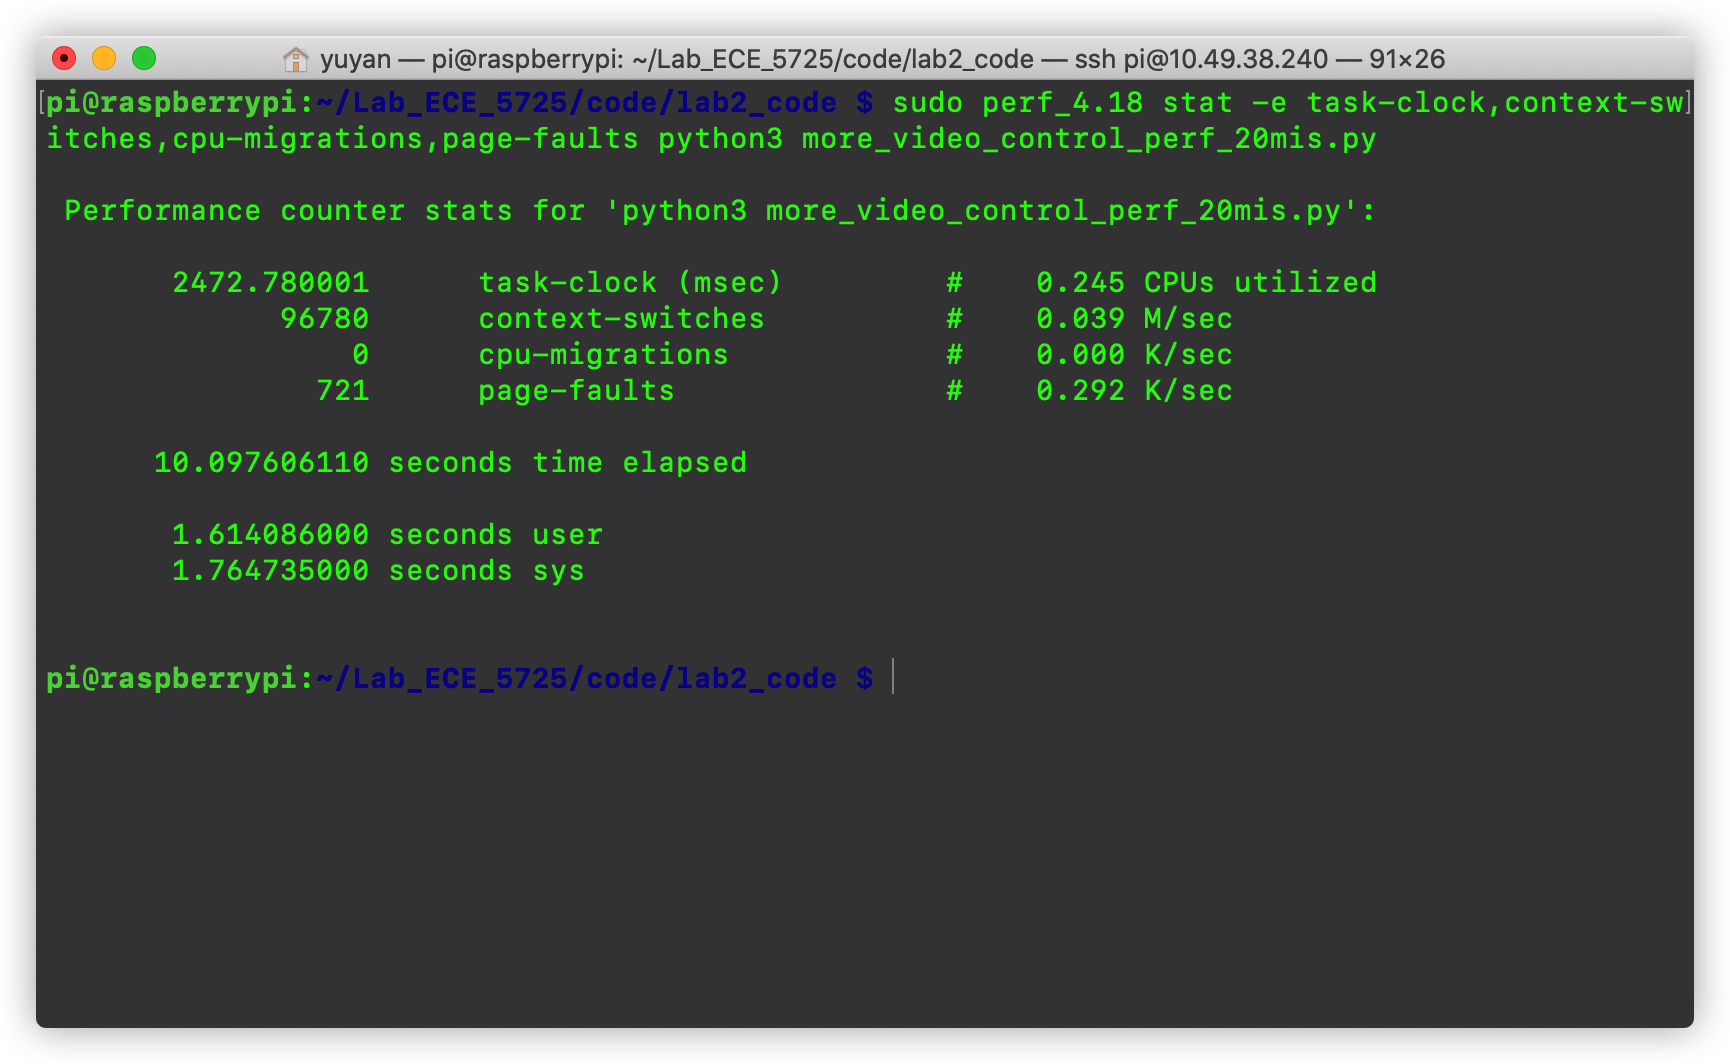
\includegraphics[width=\textwidth]{img/more_video_control_perf_20mis.png}
\caption{Performance of 20 microseconds}
\label{fig:fig7}
\end{minipage}
\end{figure}
\begin{figure}[H]
    \centering
    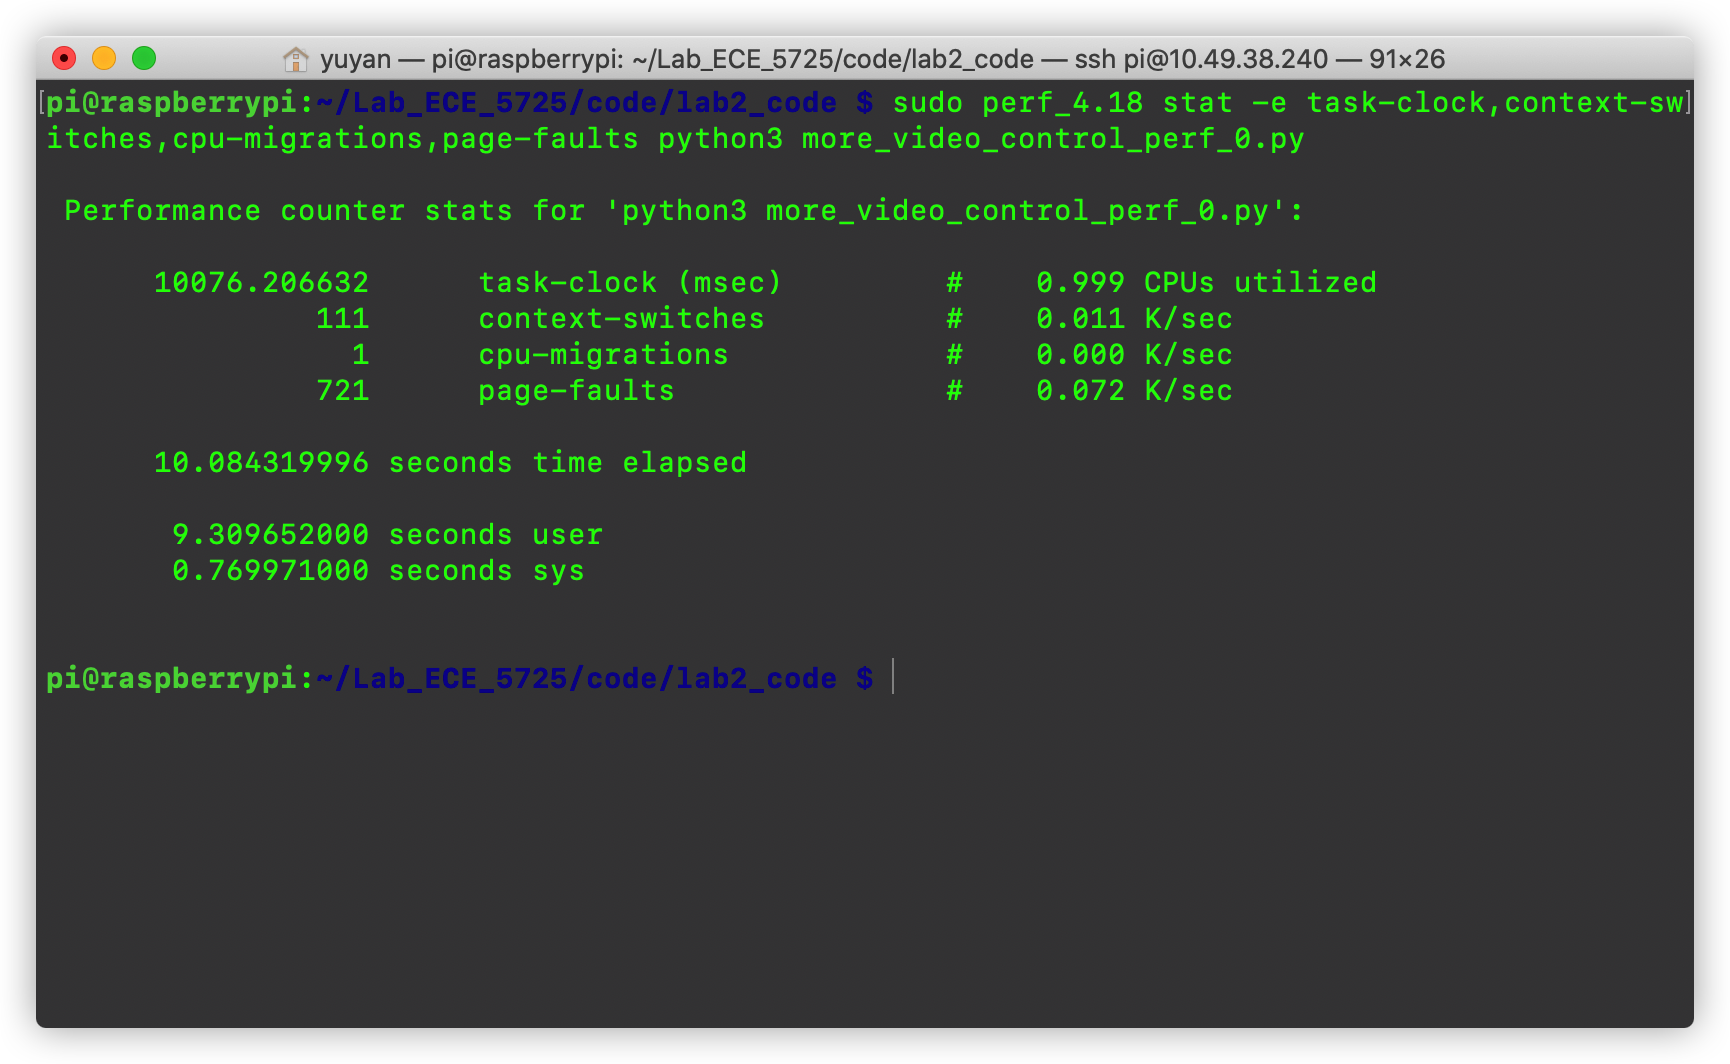
\includegraphics[width=0.5\textwidth]{img/more_video_control_perf_0.png}
    \caption{Performance of 0}
    \label{fig:fig8}
\end{figure}
I can easily find that as the polling time becomes smaller, the CPU resources occupied by program  \code{more\_video\_control.py} are rapidly increasing. When the polling time is 0, it takes up almost all of the CPU resources. This is because as the polling interval is shortened, the program \code{more\_video\_control.py} polls more and more frequently, naturally taking up more CPU resources. That's why I need to use the callback function to implement the interrupt detection. In this way, the program does not use too much CPU resources in normal times, but only switches to the callback function when the interrupt occurs and performs the operation I have defined.\vspace{-1em}

\subsection*{2.3 Pygame Programs}\vspace{-1em}
In this section, I need to complete three Python programs, including \code{bounce.py}, \code{two\_bounce.py} and \code{two\_collide.py}, with applying the Pygame library. The complete code of them are listed in the Appendix. Because their basic implementation architecture is very similar, here I do not expand on the details of the code, but rather introduce the common code logic, some of the problems encountered and the solutions. \par
First let's talk about how to represent a picture or an object with Pygame. In our code, I used the function \code{pygame.image.load()} to read the image file and then created a \code{rect} object to represent the image I got. I can initialize the position of the object by specifying the left value and the bottom value of the \code{rect} object. The example code is shown in code listing \ref{code:code4}. 
\begin{center}
\begin{lstlisting}[language=Python, caption=The example code for representing image with Pygame , label=code:code4]
import pygame 
ball_big = pygame.image.load("magic_ball.png")
ballrect_big = ball_big.get_rect()
ballrect_big.left = 192
ballrect_big.bottom = 128
\end{lstlisting}
\end{center}\vspace{-2em}
After knowing how to create our elements, let's see how to make our elements move. In other words, how to implement animations. The basic flow is shown below:\vspace{-1em}
\begin{enumerate}
    \item Create the elements and specify their initialization position as mentioned above
    \item Move the created \code{rect} object by a speed vector, like \code{ballrect\_big = ballrect\_big.move}\\\code{([1,1])}
    \item Clean the screen by re-filling the screen with background color, like \code{screen.fill(0,0,0)}
    \item Bind the image to the moved \code{rect} object and add it to the screen by using the \code{blit()} function, like \code{screen.blit(ball\_big, ballrect\_big)}
    \item Display the new frame on the screen by using the function \code{pygame.display.flip()}
\end{enumerate}\vspace{-1em}
With such flow, I can successfully make our picture move. Next, let's see how to achieve making the ball bounce back when it hits the boundary.The logic to achieve this function is actually very simple, that is, after each change in the position of the \code{rect} object, check whether the boundary is touched. If the boundary is touched, the velocity vector of the ball will be changed so that the velocity of the corresponding dimension is reversed. This way, the next motion of the ball will be in the opposite direction of the previous motion.\par
With this logic understood, I can easily complete the first two programs, \code{bounce.py} and \code{two\_boun}\\\code{ce.py}. In order to implement the last program, \code{two\_collide.py}, I also need to understand how to implement the collision detection of \code{rect} objects and use the principle of elastic collision to change the velocity of the ball after the collision.\par
The Pygame library actually has provided a function to detect if a collision has occurred on a \code{rect} object. It is \code{colliderect()}. We can use it like \code{ballrect\_big.colliderect(ballrect\_small)}. This function will return \code{True} if a collision has occurred, otherwise it will return \code{False}.\par
But in our case, there is a flaw to using this method. I hadn't noticed it, but when I showed my program to the TA, she pointed it out: because the actual area of the ball and the actual area of the \code{rect} object we used (which was in fact a square) didn't exactly match, there were times when it looked like we had detected a collision event and changed the orientation of the two balls without the two balls touching each other.\par
To fix this problem, I need to customize the conditions for collision detection. If the radius of the two balls and the location of their circle centers can be known, it is possible to determine whether the balls have collided by comparing the sum of their radius and the magnitude of the absolute distance between the location of the circle centers. After looking up Pygame's documentation, I found that I can use the \code{Rect.inflate()} method to specify the size of the \code{rect} object. In this way, the radius of the ball can be calculated. What's more, the current center position of the \code{rect} object can be obtained by calling the properties \code{Rect.centerx} and \code{Rect.centery}. Because of time constraints, I did not have time to do this optimization in this part of the experiment. However, I implemented this method in the last section of the experiment.\par
As for updating the speed of the ball after the collision, because of my very poor mathematical and physical ability, I did not use the principle of elastic collision to calculate the new speed, but directly and simply let the ball obtain the speed in the opposite direction from its original speed after the collision.\par
There is still one more thing that I would like to state here.\par
In my original program running effect, the ball was moving very fast, even though I just set the speed to only 1 and 2. I was very surprised by this phenomena, but thought it was caused by the small screen size of the piTFT. When I ran this program on the monitor, the ball was moving at a relatively reasonable speed. \par
When giving the TA checkout, the TA told me that I could slow down the ball by setting \code{time.sleep(}\\\code{0.2)} in the loop. I didn't understand it very well at that time, but now I understand that the principle of this change is actually the same as the measuring performance in the section 2.2. By extending the polling interval, the refresh speed of screen would be reduced.\par
Later in the class, the professor also talked about this problem and offered an even better approach. Actually, the FPS of the Pygame program can be directly defined with the function \code{pygame.time.Clock().tick(FPS)}. This approach is very helpful for the design of the program I will introduce in the section 2.5.\par
At this point, I have completed all the requirements for week1 and was the first to checkout.\vspace{-1em}
\subsection*{2.4 piTFT Touch Control Configuration}\vspace{-1em}
For me, the process of configuring the piTFT touch went very smoothly, so I won't go into too many details of the configuration process here. Just follow the step-by-step instructions on the experimental guide to complete all the configuration work smoothly. In this section, I just want to describe a problem that came up in the experimental guide and my solution to it.\par
In the version 2 of the lab guide, there is a step that we need to create a file \code{/etc/apt/apt.conf.d/1}\\\code{0defaultRelease} to specify the version of the aimed package we want to install. To implement this requirement, we need to add a line to this file, which is \code{APT::Default-release “stable”;}. The last word in this sentence, "stable," is the root cause of the problem. \par
If you add this line to the file, then when you execute the download command later, you will get an error that the "stable" version of the package cannot be found. At the time I did the experiment, I didn't really know what was causing this version to fail. But this is a common thing inside Linux, a package can't be found probably because the naming was updated.\par
When I was doing the experiment, to solve this problem, I just removed the last word, "stable". This way you don't specify the version of the downloaded package, and as long as the package name remains the same, you should be able to install it successfully. Of course, there is no guarantee that the installed version will work properly later. However, it has since been proven that this is workable. The touch function of piTFT works normally.\par
Later, the professor told the class about the orthodox solution and the real reason. On 9.27, the version name of this package was updated. There is no longer a version named "stable". We should download the "wheezy" version of the package.\par
This lesson should be remembered. When we failed to download a package because the version cannot be found, we need to go to the official release site of the package to see what is happening. However, in the lab, we only need to make it work as soon as possible without caring about the real reason behind.\vspace{-1em}
\subsection*{2.5 Pygame Programs with piTFT Touch Control}\vspace{-1em}
In this last section, I need to combine piTFT's touch controls with my previous knowledge of Pygame to complete programs, including \code{Quit\_button.py}, \code{Screen\_coordinates.py}, \code{Two\_but}\\\code{ton.py} and the \code{Control\_two\_collide.py}.\par
First, to enable to get the touch event from the piTFT screen, some environment variables need to be clarified in the head of our Python scripts. The configuration of these environment variables is shown in the code listing \ref{code:code5}.
\begin{center}
\begin{lstlisting}[language=Python, caption=Environment variables settings, label=code:code5]
# Environment Seting
os.putenv('SDL_VIDEODRIVER', 'fbcon') # Display on piTFT
os.putenv('SDL_FBDEV', '/dev/fb0') #
os.putenv('SDL_MOUSEDRV', 'TSLIB') # Track mouse clicks on piTFT
os.putenv('SDL_MOUSEDEV', '/dev/input/touchscreen')
\end{lstlisting}
\end{center}\vspace{-2em}
After setting this up, we should have been able to rest easy as well. But things often go awry.\par
Sometimes, after restarting the Raspberry Pi, we may encounter a situation where our program does not run properly because it does not recognize the touch device. To fix this problem, we should run the code \code{fix\_touchscreen} offered by the professor.\par
Next, let's see how to detect if a button on the screen has been pressed. The principle is actually very simple.\par
First I need to know if a touch has occurred. Here, I use a function provided by Pygame, \code{pygame.eve}\\\code{nt.get()}, through which I can get the last occurred event. There are two types of events in total that I need to be concerned about. The first is \code{MOUSEBUTTONDOWN} meaning that the mouse has been pressed down. The second, more important one, is \code{MOUSEBUTTONUP} meaning that the mouse has been pressed and up. So as soon as I detect the second event, I know that a touch action has been completed.\par
The next question is how to know if the touch action pressed the key I set. In fact, there is a easy way to determine whether the touch is a key press. If I can get the position of the touch point and judge it against the area of the buttons I have set, I can then know if this touch is a button click or not.\par
By using the function \code{Pygame.mouse.get\_pos()}, the position of the touch point can be obtained. For the button area, its width, height and position can be obtained by calling its \code{rect} properties. Once these information are known, a simple judgment is all that is needed to complete the functional logic these program need.\par
As mentioned above, I have improved the collision judgement logic for this section, but still no improved the speed updateing logic.\par
At this point, all experimental procedures, problems, phenomena and solutions have been clearly stated. I was still the first one to check out for the week2.\vspace{-1em}
\newpage
\section*{3. Conclusion}\vspace{-1em}
In this experiment, I think the most important thing I learned was about the Pygame library. With Pygame and the touch screen, I believe I've been able to design and develop a lot of interesting games. Maybe my final project will be a small game based on these.\par
Besides that, the format of this experiment is very good to me, both the hardware part and the software part. The only suggestion would be to consider moving some of the Pygame programming from week1 to week 2. I think the Pygame programming fits better with the week2's content and the week1's workload is slightly more than the week2's workload.\par
Finally, I would like to thank the professors and all the TAs who were very helpful during the experiment.
\newpage
\section*{4. Code Appendix\vspace{-1em}}
\begin{center}
\lstinputlisting[language=Python, caption=six\_button.py]{code/sixbuttons.py}
\end{center}\vspace{-2em}

\begin{center}
\lstinputlisting[language=Python, caption=more\_video\_control.py]{code/more_video_control.py}
\end{center}\vspace{-2em}

\begin{center}
\lstinputlisting[language=Python, caption=start\_video]{code/start_video.sh}
\end{center}\vspace{-2em}

\begin{center}
\lstinputlisting[language=Python, caption=more\_video\_control\_cb.py]{code/more_video_control_cb.py}
\end{center}\vspace{-2em}

\begin{center}
\lstinputlisting[language=Python, caption=start\_video\_cb]{code/start_video_cb.sh}
\end{center}\vspace{-2em}

\begin{center}
\lstinputlisting[language=Python, caption= more\_video\_control\_perf.py]{code/more_video_control_perf.py}
\end{center}\vspace{-2em}

\begin{center}
\lstinputlisting[language=Python, caption=more\_video\_control\_cb\_perf.py]{code/more_video_control_cb_perf.py}
\end{center}\vspace{-2em}

\begin{center}
\lstinputlisting[language=Python, caption=bounce.py]{code/bounce.py}
\end{center}\vspace{-2em}

\begin{center}
\lstinputlisting[language=Python, caption=two\_bounce.py]{code/two_bounce.py}
\end{center}\vspace{-2em}


\begin{center}
\lstinputlisting[language=Python, caption=two\_collide.py]{code/two_collide.py}
\end{center}\vspace{-2em}

\begin{center}
\lstinputlisting[language=Python, caption=Quit\_button.py]{code/Quit_button.py}
\end{center}\vspace{-2em}

\begin{center}
\lstinputlisting[language=Python, caption=Screen\_coordinates.py]{code/screen_coordinates.py}
\end{center}\vspace{-2em}

\begin{center}
\lstinputlisting[language=Python, caption=Two\_button.py]{code/two_buttons.py}
\end{center}\vspace{-2em}

\begin{center}
\lstinputlisting[language=Python, caption=Control\_two\_collide.py]{code/control_two_collide.py}
\end{center}\vspace{-2em}



% To add math, use
%\begin{equation}
 %Helpful links    https://www.overleaf.com/learn/latex/Mathematical_expressions
%\end{equation}

%To add hyperlinks, use 
%For further references see \href{http://www.overleaf.com}{Something Linky} or go to the next url: \url{http://www.overleaf.com}

% It's also possible to link directly any word or \hyperlink{thesentence}{any sentence} in you document.

% Tables 

% \begin{table}[h!]
% \centering
%  \begin{tabular}{||c c c c||} 
%  \hline
%  Col1 & Col2 & Col2 & Col3 \\ [0.5ex] 
%  \hline\hline
%  1 & 6 & 87837 & 787 \\ 
%  2 & 7 & 78 & 5415 \\
%  3 & 545 & 778 & 7507 \\
%  4 & 545 & 18744 & 7560 \\
%  5 & 88 & 788 & 6344 \\ [1ex] 
%  \hline
%  \end{tabular}
% \end{table}

% Images

% upload your images to the img folder. To print them in the document, uncomment the following
% \begin{figure}[h]
%     \centering
%     \includegraphics[width=0.25\textwidth]{/img/YourImageTitle}
%     \caption{a nice plot}
%     \label{fig:mesh1}
% \end{figure}

% As you can see in the figure \ref{fig:mesh1}, the 
% function grows near 0. Also, in the page \pageref{fig:mesh1} 
% is the same example.
\newpage
\printbibliography

\end{document}
